
\documentclass{article} % Don't change this

\usepackage{tabularx} % extra features for tabular environment
\usepackage{amsmath}  % improve math presentation
\usepackage{graphicx} % takes care of graphic including machinery
\usepackage[margin=1.25in,letterpaper]{geometry} % decreases margins
\usepackage{cite} % takes care of citations
\usepackage{subfigure}
\usepackage{float}    % For tables and other floats
\usepackage[final]{hyperref} % adds hyper links inside the generated pdf file
\usepackage{listings}
\usepackage[framed,numbered,autolinebreaks,useliterate]{mcode}
\usepackage{lipsum}
\usepackage{appendix}
\usepackage{cite}
\hypersetup{
	colorlinks=true,       % false: boxed links; true: colored links
	linkcolor=blue,        % color of internal links
	citecolor=blue,        % color of links to bibliography
	filecolor=magenta,     % color of file links
	urlcolor=blue         
}
\newcommand{\blah}{blah blah blah \dots}



\setlength{\marginparwidth}{3.4cm}

% NEW COUNTERS
\newcounter{points}
\setcounter{points}{100}
\newcounter{spelling}
\newcounter{usage}
\newcounter{units}
\newcounter{other}
\newcounter{source}
\newcounter{concept}
\newcounter{missing}
\newcounter{math}

% COMMANDS
%\newcommand{\raisa}[2]{\colorbox{Yellow}{#1} \todo{#2}}
\newcommand{\arbitrary}[2]{\todo{#1 #2} \addtocounter{points}{#2} \addtocounter{other}{#2}}
\newcommand{\english}{\todo{LANGUAGE (-1)} \addtocounter{points}{-1}
\addtocounter{usage}{-1}}
\newcommand{\units}{\todo{UNITS (-1)} \addtocounter{points}{-1}
\addtocounter{units}{-1}}
\newcommand{\spelling}{\todo{SPELLING and GRAMMAR (-1)} \addtocounter{points}{-1}
\addtocounter{spelling}{-1}}
\newcommand{\source}{\todo{SOURCE(S) (-2)} \addtocounter{points}{-2}
\addtocounter{source}{-2}}
\newcommand{\concept}{\todo{CONCEPT (-2)} \addtocounter{points}{-2}
\addtocounter{concept}{-2}}
\newcommand{\missing}[2]{\todo{MISSING CONTENT (#1) #2} \addtocounter{points}{#1}
\addtocounter{missing}{#1}}
\newcommand{\maths}{\todo{MATH (-1)} \addtocounter{points}{-1}
\addtocounter{math}{-1}}

\newcommand{\summary}[1]{
\begin{mdframed}[nobreak=true]
\begin{minipage}{\textwidth}
\vspace{0.5cm}
\begin{center}
\Large{Grade Summary} \hrule 
\end{center} \vspace{0.5cm}
General Comments: #1

\vspace{0.5cm}
Possible Points \dotfill 100 \\
Points Lost (Spelling and Grammar) \dotfill \thespelling \\
Points Lost (Language) \dotfill \theusage \\
Points Lost (Units) \dotfill \theunits \\
Points Lost (Math) \dotfill \themath \\
Points Lost (Sources) \dotfill \thesource \\
Points Lost (Concept) \dotfill \theconcept \\
Points Lost (Missing Content) \dotfill \themissing \\
Other \dotfill \theother \\[0.5cm]
\begin{center}
\large{\textbf{Grade:} \fbox{\thepoints}}
\end{center}
\end{minipage}
\end{mdframed}}

%#########################################################

%To use symbols for footnotes
\renewcommand*{\thefootnote}{\fnsymbol{footnote}}
%To change footnotes back to numbers uncomment the following line
%\renewcommand*{\thefootnote}{\arabic{footnote}}

% Enable this command to adjust line spacing for inline math equations.
% \everymath{\displaystyle}

% _______ _____ _______ _      ______ 
%|__   __|_   _|__   __| |    |  ____|
%   | |    | |    | |  | |    | |__   
%   | |    | |    | |  | |    |  __|  
%   | |   _| |_   | |  | |____| |____ 
%   |_|  |_____|  |_|  |______|______|
%%%%%%%%%%%%%%%%%%%%%%%%%%%%%%%%%%%%%%%

\title{
\normalfont \normalsize 
\textsc{Rutgers University \\ 
Summer Research Program} \\
[10pt] 
\rule{\linewidth}{0.5pt} \\[6pt] 
\huge Algorithm Recurrence of First Paper  \\
\rule{\linewidth}{2pt}  \\[10pt]
}
\author{Han Liu}
\date{\normalsize \today}

\begin{document}

\maketitle



\section{Introduction}
In the process of training and predicting a gaussian process (GP), we need to get three quantities: the mean of predicted input, the log marginal likelihood function and its derivative. Their expressions are given as following:
\begin{equation}
u_{f|D}(\hat{x})=u(\hat{x})+k_{X\hat{x}}^{T}K^{-1}y
\end{equation}

\begin{equation}\label{eq1}
logp({y|K})=-\frac{1}{2}log((2\pi)^k|K|)-\frac{1}{2}y^T{K}^{-1}y
\end{equation}

\begin{equation}
\frac{\partial}{\partial \theta_j}logp(y|X,\theta)=\frac{1}{2}y^{T}K^{-1}\frac{\partial K}{\partial \theta_j}K^{-1}y-\frac{1}{2}tr(K^{-1}\frac{\partial K}{\partial \theta_j})
\end{equation}
These equation have three operations in common that dominate its time complexity: $K^{-1}y$, $log|K|$, $tr(K^{-1}\frac{\partial K}{\partial \theta_j})$. Before that, I use Cholesky decomposition of $K$ to compute all three quantities (see $GP\_code.py$), but it is very computational expensive, thus we need some parallel computional algorithm.\\
I think the innovative part of this paper is to use matrix-matrix multipy to combine three algorithms (Conjugate Gradient, Lancos Algorithm, Pivoted Cholesky Decomposition) together. The most important formula is as following:
\begin{equation}\label{equ1}
[u_0 \quad u_1 \quad ... \quad u_t]=K^{-1}[y \quad z_1 \quad ... \quad z_t]
\end{equation}
The whole algorithm flow chart can be seen in Figure \ref{fig1}. In the following section, I will implement all the three algorithms individually by MATLAB.

 \begin{figure}[h]
	\begin{center}
		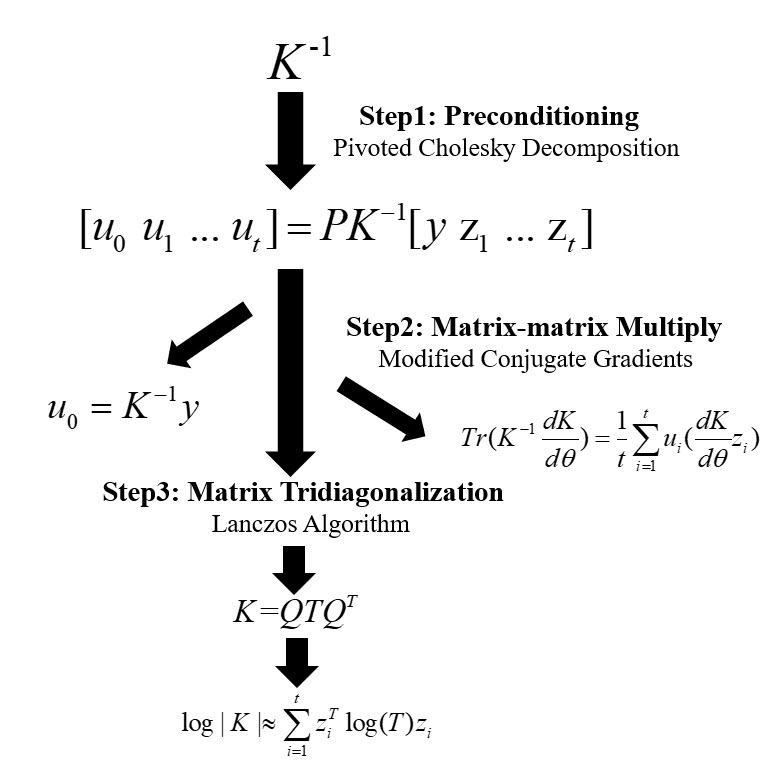
\includegraphics[width=0.6\textwidth]{algorithm}
	\end{center}
	\caption{Overall Algorithm Flow Chart}
	\label{fig1}
\end{figure}

\section{Implementation of mBCG}
In this section, I firstly implement standard preconditioned conjugate gradient algorithm, then I try to implement modified conjugate gradient algorithm given in Equation \ref{equ1}. 
\subsection{Standard PCG}
For the implementation of standard preconditioned conjugate gradient (PCG), I carefully follow the \textbf{Algorithm 1} in the paper. But unfortunately, I failed to get the correct results. It bothered me almost entire day, and I refer many literature, and try to implement this algorithm in a different dimension. For example, \textbf{Conjugate Gradient Method} [1] from Stanford University specify the process as following: 

 \begin{figure}[H]
	\begin{center}
		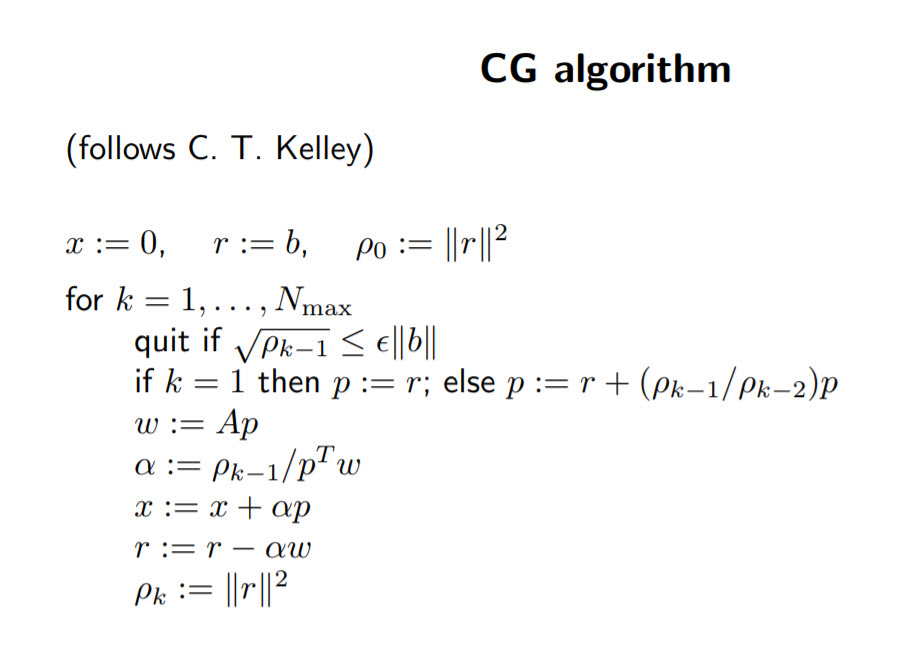
\includegraphics[width=0.55\textwidth]{CG}
	\end{center}
	\caption{Conjugate Gradient Method}
	\label{fig2}
\end{figure}
The MATLAB code is given in $PCG\_stanford.m$. Finally, I found there are two mistakes in the paper, which can be seen in the following figure:

 \begin{figure}[H]
	\begin{center}
		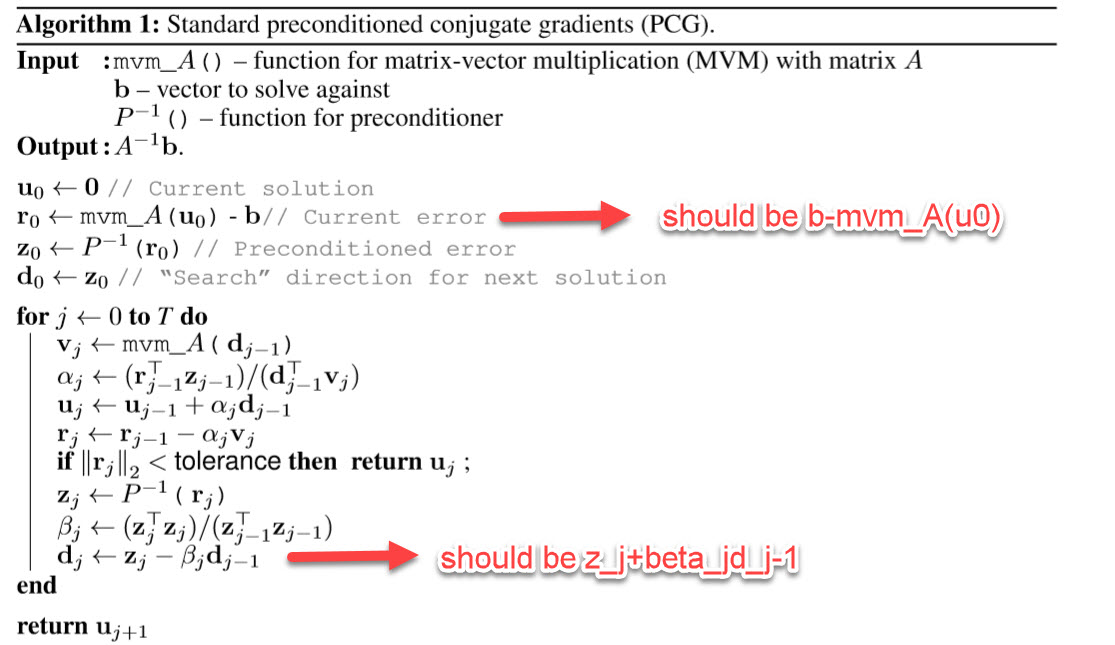
\includegraphics[width=0.65\textwidth]{PCG}
	\end{center}
	\caption{Correction of PCG Algorithm}
	\label{fig3}
\end{figure}
A simple test for the following input is given in Figure \ref{fig4}:
\begin{equation}
A={
	\left[ \begin{array}{ccc}
	6 & 3 & 0\\
	3 & 6 & -6\\
	0 & -6 & 11
	\end{array} 
	\right ]},
b={
	\left[ \begin{array}{ccc}
	3 \\
	1\\
	2 
	\end{array}
	\right ]}
\end{equation}

 \begin{figure}[H]
	\begin{center}
		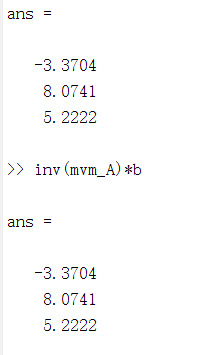
\includegraphics[width=0.35\textwidth]{test2}
	\end{center}
	\caption{Matlab Test Results}
	\label{fig4}
\end{figure}


\subsection{Modified PCG}
To implement a modified (batched) PCG, we need to convert MVM to MMM. There are several modifications of original algrithm, and some proofs are given in appendix. The MATLAB code is as following:
\begin{lstlisting}
%Modified preconditioned conjugate gradients

mmm_A=  [ -3.3704    0.2593   -3.6296;
8.0741    0.4815    7.9259;
5.2222    0.4444    4.7778];
B=[4 3 2;7 1 8;9 2 5];
col=size(B,2);
U=zeros(3,3);
R=B-mmm_A*U;
Z=R;
D=Z;
alpha=zeros(3,1);
beta=zeros(3,1);
t=3;        %number of iteration
e=0.0001;

for j=1:3
	V=mmm_A*D;
	alpha=(dot(R,Z)./dot(D,V))';
	U= (U'+diag(alpha)*D')';
	R= (R'-diag(alpha)*V')';
	norm_matrix=zeros(1,col);
	for i=1:col
		norm_matrix(i)=norm(R(:,i),2);
	end
	if any(any(norm_matrix<e))
		break
	end
	Z_old=dot(Z,Z);
	Z=R;
	beta=(dot(Z,Z)./Z_old)';
	D=(Z'+diag(beta)*D')';
end
display(U)
\end{lstlisting}






\section{Implementation of Lanczos Algorithm}
To implement Lanczos Algorithm for tridiagonalizing a symmetric matrix A, I refer the alogorithm given in \textbf{Algorithm 2}. Specifically,
we have:\\
\begin{equation}
\begin{aligned}
\forall i \quad [T_i]_{j,j}=1/[\alpha_j]_i+[\beta_{j-1}]_i/[\alpha_{j-1}]_i \\
[T_i]_{j-1,j}, [T_i]_{j,j-1}=\sqrt{[\beta_{j-1}]}/[\alpha_{j}]_i \\
\end{aligned}
\end{equation}
I have implemented this algorithm in MATLAB as following:
\begin{lstlisting}
function [ T ] = Lanczos_Algorithm( alpha,beta )
	col=size(alpha,2);  %iteration
	row=size(alpha,1);  %third-dimension of T
	T=zeros(col,col,row);
	for i=1:row
		for j=1:col
			if j==1
				T(1,1,i)=1/alpha(i,1);
			else
				T(j,j,i)=1/alpha(i,j)+beta(i,j-1)/alpha(i,j-1);
				T(j-1,j,i)=sqrt(beta(i,j-1))/alpha(i,j-1);
				T(j,j-1,i)= T(j-1,j,i);
			end
		end
	end
end
\end{lstlisting}
To test the correctness of this algorithm, I have choose two matrixes:
\begin{equation}
\alpha={
	\left[ \begin{array}{ccc}
	6 & 3 & 1\\
	3 & 2 & -6\\
	1 & -6 & 11
	\end{array} 
	\right ]},
\beta={
	\left[ \begin{array}{ccc}
	1 & 2 & 3\\
	3& 4 & 5\\
	6 & 7 & 8
	\end{array}
	\right ]}
\end{equation}
The calculation results from calculator and program operation results are as following:
\begin{figure}[H]
	\centering
	\subfigure[MATLAB Results]{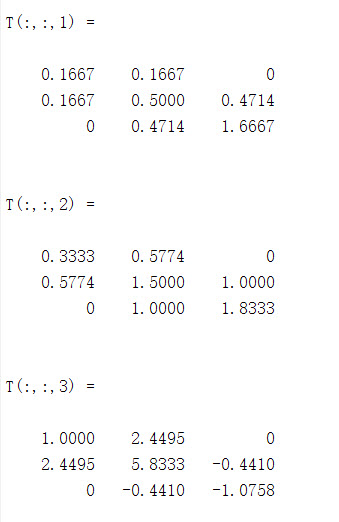
\includegraphics[width=2.7in]{matlab}}
	\subfigure[Calculator Results]{\includegraphics[width=2.7in]{test}}
	\caption{Comparison of Two Implementations}
	\label{fig2}
\end{figure}

\section{Implementation of Pivoted Cholesky Decomposition}
The preconditioning is an operation of utilizing hardware more efficiently. In this paper, the author use \textbf{Pivoted Cholesky Decomposition (PCG)}. Specifically, PCG algorithm will produce a low-rank approximation of a positive definite matrix, which is:
\begin{equation}
K_{XX}=L_kL_k^T
\end{equation} 
The pseudo-code of PCG algorithm is as following [2]:

 \begin{figure}[H]
	\begin{center}
		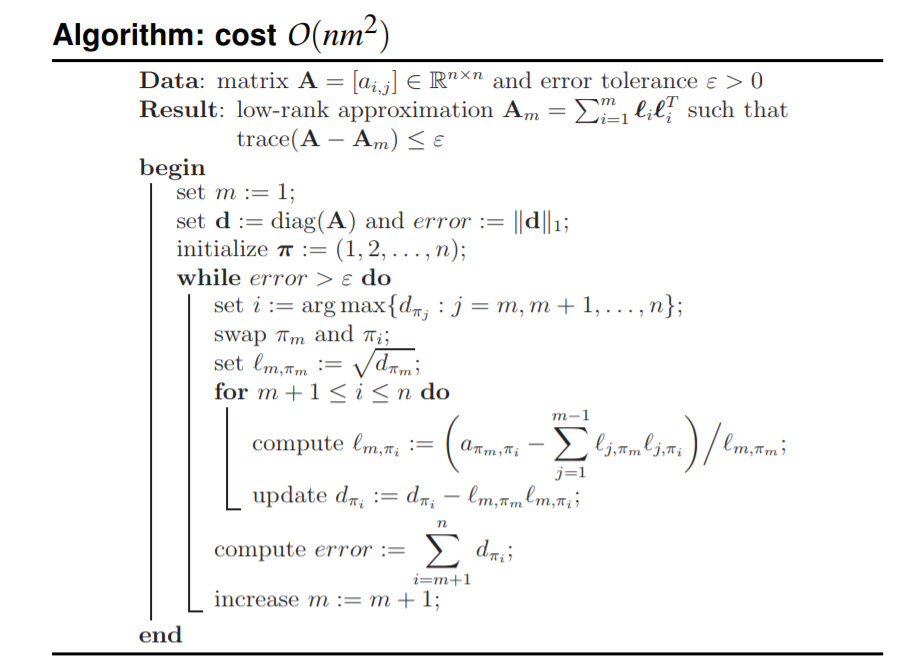
\includegraphics[width=0.85\textwidth]{PCD}
	\end{center}
	\caption{Pivoted Cholesky Decomposition Algorithm}
	\label{fig2}
\end{figure}
I implement this algorithm by MATLAB:

\begin{lstlisting}
%Implementation of Pivited Cholesky Composition
A=[6 3 0;
3 6 -6;
0 -6 11];    %semi-positive matrix

e=0.1;            %Error
n=size(A,1);

m=1;
d=diag(A);
error=norm(d,1);
v=randperm(n);
Pi = sort(v);
l=zeros(n,n);   %triangular matrix we want 

while error>e
	[argvalue, i] = max(d(Pi(m:end)));
	a=Pi(m);
	Pi(m)=Pi(i);
	Pi(i)=a;
	l(m,Pi(m))=sqrt(d(Pi(m)));
	for i = (m+1:n)
		S=0;
		for j =(1:m-1)
			l(j,Pi(m))
			l(j,Pi(i))
			S=S+l(j,Pi(m)).*l(j,Pi(i));
		end
		l(m,Pi(i))=(A(Pi(m),Pi(i))-S)./l(m,Pi(m));
		d(Pi(i))=d(Pi(i))-l(m,Pi(m)).*l(m,Pi(i));
	end
%compute error
	error_s=0;
	for i = (m+1:n)
		error_s=error_s+d(Pi(i));
	end
	error=error_s;
	m=m+1;      
end

S_Am=zeros(3,3);
for i=(1:m-1)
	S_Am=S_Am+l(:,i)*l(:,i)';
end
Am=S_Am;

\end{lstlisting}

\begin{thebibliography}{1}
	
	\bibitem{1}https://stanford.edu/class/ee364b/lectures/conj\_grad\_slides.pdf
	\bibitem{2}Helmut Harbrecht, Michael Peters, and Reinhold Schneider, "The pivoted Cholesky decomposition
	and its application to stochastic PDEs", p7.
	http://www.mathe.tu-freiberg.de/naspde2010/sites/default/files/harbrecht.pdf
\end{thebibliography}
\begin{appendices}
\section{Derivation of mBCG}
 \begin{figure}[H]
	\begin{center}
		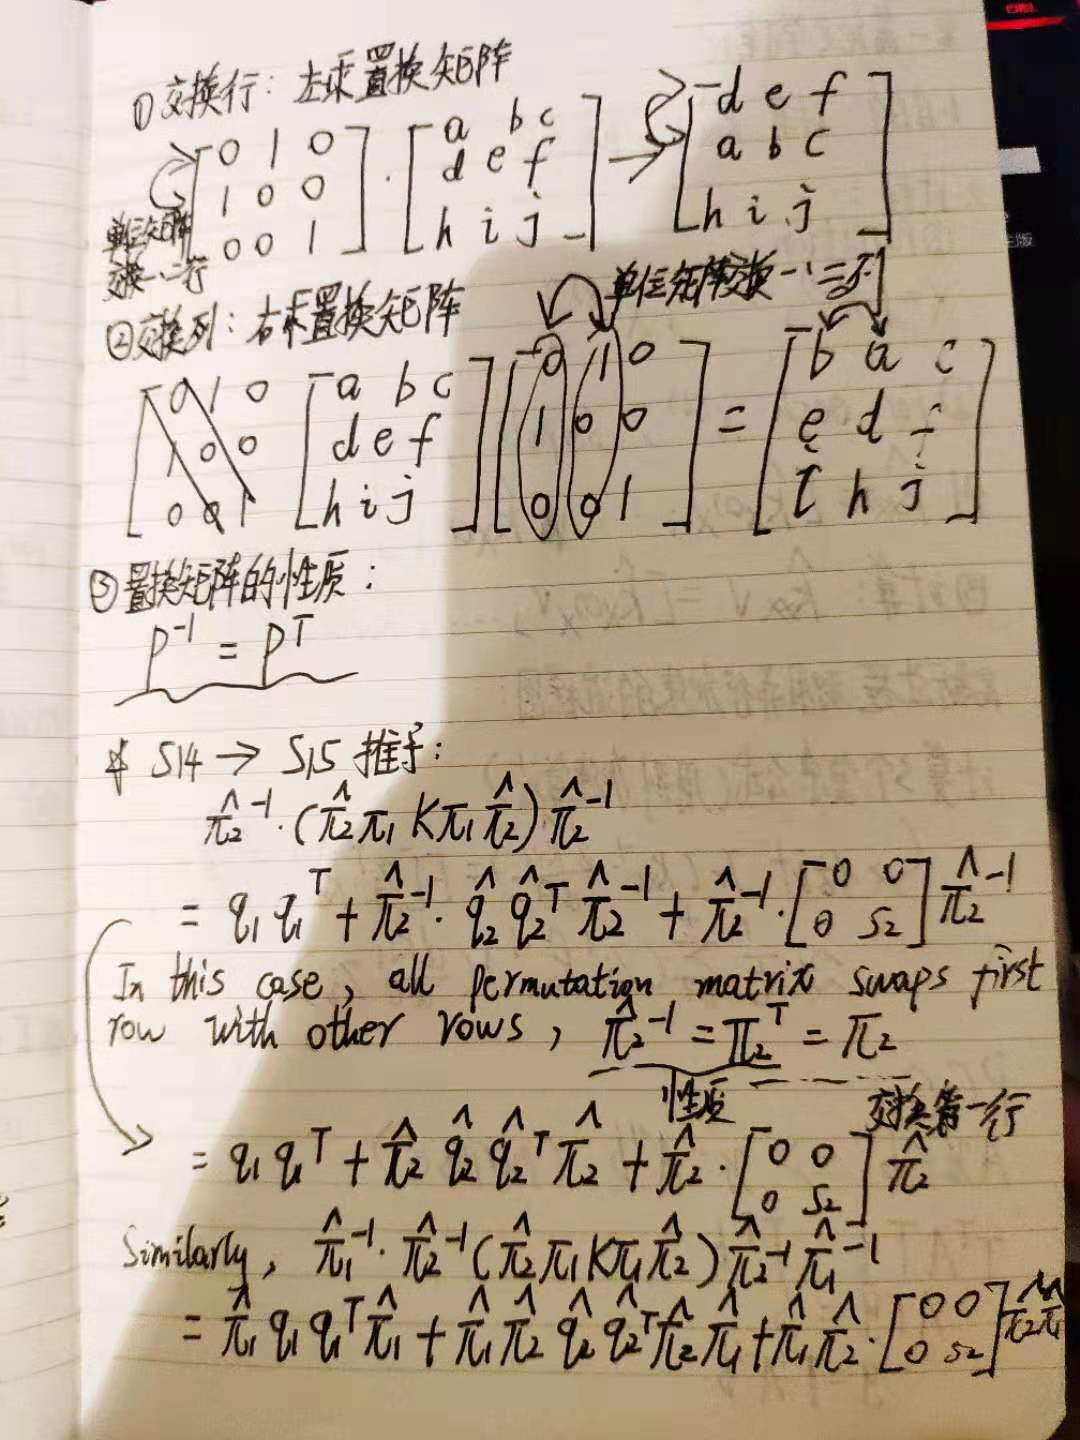
\includegraphics[width=0.85\textwidth]{111}
	\end{center}
	\caption{Derivation of mBCG}
	\label{fig2}
\end{figure}
\end{appendices}




\end{document} % NOTHING AFTER THIS LINE IS PART OF THE DOCUMENT
